\documentclass[12pt, a4paper]{ctexart}
\usepackage{graphicx}
\usepackage{indentfirst, amsmath}
\usepackage{tikz}
\usepackage{fancyhdr}
\pagestyle{fancy}
\lhead{}
\rhead{}
\chead{\fangsong 概率论实验报告} 
\cfoot{}
\rfoot{\thepage} 
\renewcommand{\headrulewidth}{0.4pt} 
\renewcommand{\footrulewidth}{0pt}
\usepackage{tcolorbox,tabu}
\tcbuselibrary{listings,theorems,skins}
\newcommand{\exercise}[1]{\noindent\tcbox[on line,top=0mm,bottom=0mm,%
	right=0mm,left=0mm]{\bfseries 练习#1}\ }
\newcommand{\note}{\noindent\textbf{注记}\ }
\newcommand{\solve}{\newline\noindent\textbf{解}\ }


\usepackage{listings}
\usepackage[framed, numbered]{matlab-prettifier}
\lstset{language=Matlab}

\title{概率论实验报告}
\author{自动化钱71   吴思源   217131084}

\begin{document}
%%%%%%%%%%%%%%%%%%%%%%%%%%%%%%
%% 封面部分
%%%%%%%%%%%%%%%%%%%%%%%%%%%%%%
\begin{titlepage}
	\centering
	
\includegraphics[width=1.0\textwidth]{./templates/logo.png}\par
	\vspace{3.5cm}
	{\fontsize{30pt}{\baselineskip}\heiti 概率论实验报告\par}
	\vspace{2cm}
	{\fangsong\Large\itshape 吴思源\par}
	\vfill
	{2171310846}\par
	\fangsong{自动化钱71}
	\vfill
% Bottom of the page
	{\large \today\par}
\end{titlepage}

\maketitle

\section{实验一~~常见分布的概率密度、分布函数生成}

\textbf{[实验目的]}
\begin{enumerate}
	\item 会利用MATLAB软件计算离散型随机变量的概率,连续型随机变量概率密度值。
	\item 会利用MATLAB软件计算分布函数值,或计算形如事件$\left\{X\le x\right\}$的概率。
.	\item 会求上$\alpha$分位点以及分布函数的反函数值。
\end{enumerate}

\textbf{[实验要求]}
\begin{enumerate}
	\item [1]掌握常见分布的分布律和概率密度的产生命令,如binopdf,normpdf
	\item [2]掌握常见分布的分布函数命令,如 binocdf,normcdf
	\item [3]掌握常见分布的分布函数反函数命令,如binoinv,norminv
	
\end{enumerate}

\subsection{第五题}
\exercise{第五题}
设随机变量X服从均值是6,标准差是2的正态分布,求\par
(1) $X=3,4,5,6,7,8,9$ 时的概率密度值;\par
(2) $X =3,4,5,6,7,8,9 $ 时的分布函数值;\par
(3) 若$ P{X}=0.345 $,求$ X $;\par
(4) 求标准正态分布的上0.05分位数。\par

求解代码如下:

\begin{lstlisting}[style=Matlab-editor]
>> normpdf(3:9, 6, 2)  % 求解第一问概率密度
Ans = 
0.0648    0.1210    0.1760    0.1995    0.1760    0.1210    0.0648
>> nromcdf(3:9, 6, 2)  % 求解第二问分布函数值
Ans = 
0.0668    0.1587    0.3085    0.5000    0.6915    0.8413    0.9332
>> norminv(0.345, 6, 2)  % 求解第三问
Ans = 
5.2023
>> norminv(0.95, 0, 1)  % 求解分位数
Ans = 
1.6449
\end{lstlisting}


\subsection{第七题}
\exercise{第七题}
设随机变量X服从自由度是6$ \chi ^2 $分布 ,求\par
(1) X=0,1,2,3,4,5,6时的概率密度值; \par
(2) X=0,1,2,3,4,5,6时的分布函数值;\par
(3) 若$ P\left\{X\right\}=0.345 $,求$ x $;\par
(4) 求$ \chi^2 $分布的上0.05分位数.\par

求解代码如下

\begin{lstlisting}[style=Matlab-editor]
chi2pdf(0:6, 6)  % 求解第一问概率密度
Ans = 
0    0.0379    0.0920    0.1255    0.1353    0.1283    0.1120
chi2cdf(0:6, 6)  % 求解第二问分布函数值
Ans = 
0    0.0144    0.0803    0.1912    0.3233    0.4562    0.5768
chi2inv(0.345,6 )  % 求解第三问
Ans = 
4.1603
chi2inv(0.95, 6)  % 求解分位数
Ans = 
12.5916
\end{lstlisting}


\section{实验二~~概率作图}

\textbf{[实验目的]}
\begin{enumerate}
	\item 熟练掌握MATLAB软件的关于概率分布作图的基本操作
	\item 会进行常用的概率密度函数和分布函数的作图
	\item 会画出分布律图形
\end{enumerate}

\textbf{[实验要求]}
\begin{enumerate}
	\item 掌握MATLAB画图命令plot
	\item 掌握常见分布的概率密度图像和分布函数图像的画法
\end{enumerate}

\subsection{二项分布}

绘制二项分布图像$B(10, 0.3)$,代码如下:
\begin{lstlisting}[style=Matlab-editor]
%% 画出X的分布律图形;
>> x=0:10;
>> y=binopdf(x,10,0.3);
>> plot(x,y,'.')
%% 画X的分布函数图形
>> x=0:0.01:10;
>> y=binocdf(x,10,0.3);
>> plot(x,y)

\end{lstlisting}
做出图如下所示:
\begin{figure}[htbp]
	\centering
	\begin{minipage}[t]{0.48\textwidth}
		\centering
		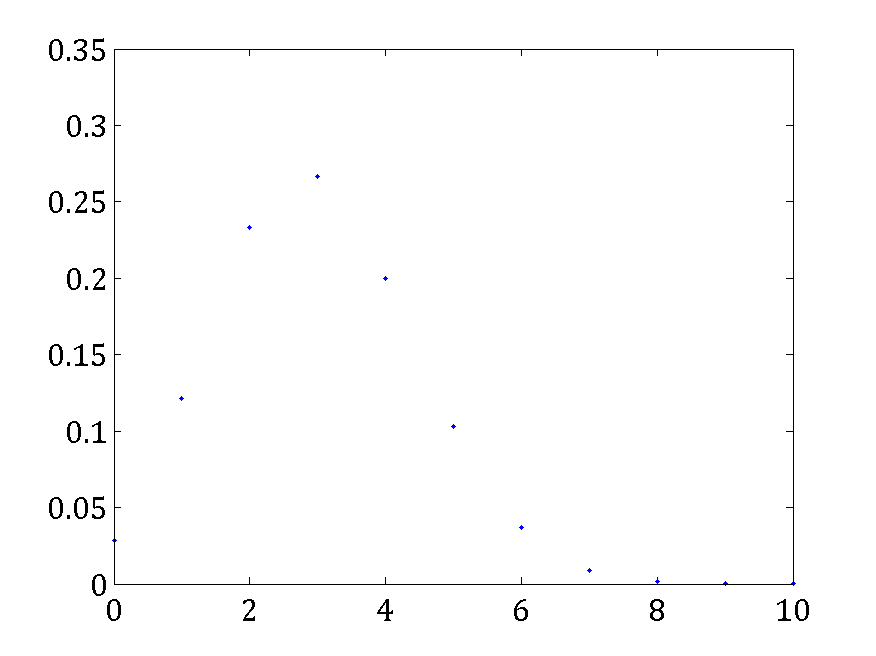
\includegraphics[width=6cm]{p1.png}
		\caption{二项分布分布律图形}
	\end{minipage}
	\begin{minipage}[t]{0.48\textwidth}
		\centering
		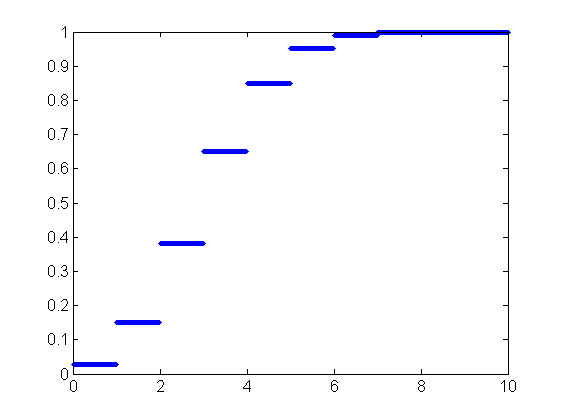
\includegraphics[width=6cm]{p2.png}
		\caption{二项分布分布函数图形}
	\end{minipage}
\end{figure}

\subsection{指数分布图像}

绘制指数分布$ exp(6) $图像代码如下:
\begin{lstlisting}[style=Matlab-editor]
%% 画出X的概率密度图形
>> x=0:0.01:10;
>> y=exppdf(x,6);
>> plot(x,y)
%% 画出X的分布函数图形
>> x=-1:0.01:10;
>> y=expcdf(x,6);
>> plot(x,y)

\end{lstlisting}
做出图如下所示:
\begin{figure}[ht]
	\centering
	\begin{minipage}[t]{0.48\textwidth}
		\centering
		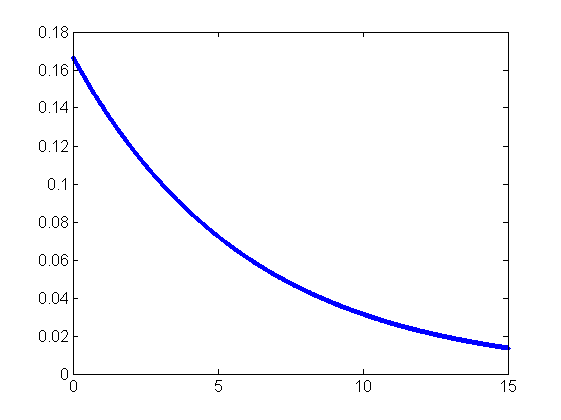
\includegraphics[width=6cm]{p3.png}
		\caption{指数分布分布律图形}
	\end{minipage}
	\begin{minipage}[t]{0.48\textwidth}
		\centering
		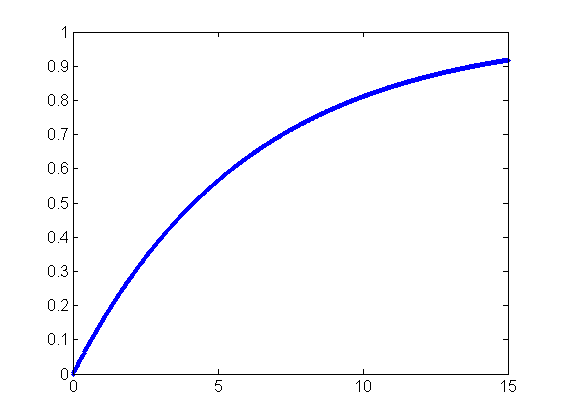
\includegraphics[width=6cm]{p4.png}
		\caption{指数分布分布函数图形}
	\end{minipage}
\end{figure}


\subsection{F分布}

绘制第一自由度是6,第二自由度是6的F分布的图像代码如下:
\begin{lstlisting}[style=Matlab-editor]
%% 画出X的概率密度图形
>> x=0:0.01:10;
>> y=fpdf(x,6);
>> plot(x,y)
%% 画出X的分布函数图形
>> x=0:0.01:10;
>> y=fcdf(x,6);
>> plot(x,y)
\end{lstlisting}
做出图如下所示:
\begin{figure}[ht]
	\centering
	\begin{minipage}[t]{0.48\textwidth}
		\centering
		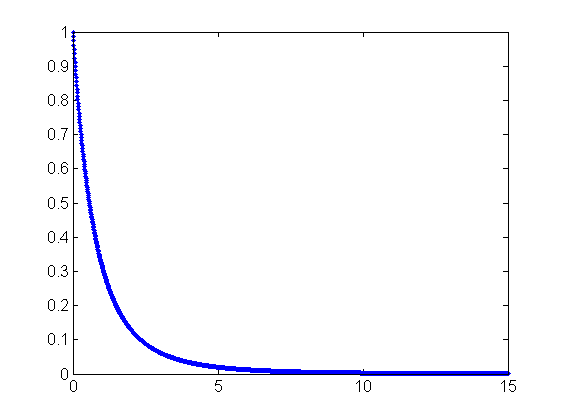
\includegraphics[width=6cm]{f6.png}
		\caption{F分布分布律图形}
	\end{minipage}
	\begin{minipage}[t]{0.48\textwidth}
		\centering
		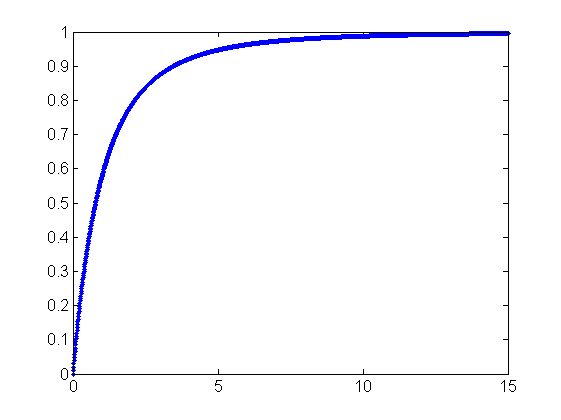
\includegraphics[width=6cm]{f5.png}
		\caption{F分布分布函数图形}
	\end{minipage}
\end{figure}

\section{实验三~~数字特征}

\textbf{[实验目的]}
\begin{enumerate}
	\item 加深对数学期望,方差的理解
	\item 理解数学期望,方差的意义,以及具体的应用
	\item 加深对协方差,相关系数的理解
	\item 了解协方差,相关系数的具体的应用
\end{enumerate}

\textbf{[实验要求]}
\begin{enumerate}
	\item  概率与频率的理论知识,MATLAB软件
	\item  协方差,相关系数的理论知识,MATLAB命令cov,corrcoef
\end{enumerate}

\subsection{第一题}
\exercise{1} 概率密度函数为
\[
f(x,y) = \left\lbrace \begin{array}{cc}
\frac{1}{2}e^{-y} & 0 \leq x \leq 2, ~ y  , \\
0, & otherwise \\
\end{array} \right.
\]
求解 $P\{X + Y \le 1\}; E(XY), E(X), E(X^2)$ 。
\solve 在MATLAB函数编辑器中写入如下代码
\begin{lstlisting}[style=Matlab-editor]
syms x y
f1 = 0.5 * exp(-y)
Pxy = int(int(f1, y, 0, 1-x), x, 0, 1)
EX = int(int(x * f1, y, 0, inf), x, 0, 2)
EX2 = int(int(x^2 * f1, y, 0, inf), x, 0, 2)
EXY = int(int(x * f1, y, 0, inf), x, 0, 2)
\end{lstlisting}

输出为
\begin{lstlisting}[style=Matlab-editor]
f1 =
1/(2*exp(y))
Pxy =
1/(2*exp(1))
EX =
1
EX2 =
4/3
EXY =
1
\end{lstlisting}

\subsection{第二题}
\exercise{2}
二维随机变量的$ (X,Y) $概率密度为
\[
f(x,y) = \left\lbrace \begin{array}{cc}
\frac{1}{3}(x + y) & 0 \leq x \leq 2, ~0 \leq y \leq 1, \\
0, & otherwise \\
\end{array} \right.
\]

计算出$ D(X) $,$ D(Y) $,$ E(XY) $,$ D(2X-3Y+8) $
\solve 在MATLAB函数编辑器中写入如下代码:
\begin{lstlisting}[style=Matlab-editor]
syms x y
int(x*y)
Ex = int(int(x * 1/3 * (x + y), 0, 2), 0, 1)
Ey = int(int(y * 1/3 * (x + y), y, 0, 1), 0, 2)
EX2 = int(int(x^2 * 1/3 * (x + y), 0, 2), 0, 1)
EY2 = int(int(y^2 * 1/3 * (x + y), y, 0, 1), 0, 2)
DX = EX2 - Ex^2
DY = EY2 - Ey^2
EXY = int(int(y * x * 1/3 * (x + y), y, 0, 1), 0, 2)
D = 4 DX + 9 DY
\end{lstlisting}

求得\par

\begin{tabular}{cccc|cccc}
	\hline
 $ E(X) $&$ E(Y) $ &$ E(X^2) $ &$ E(Y^2) $ & $ D(X) $&$ D(Y) $ & $ E(XY) $&$ D(2X-3Y+8) $ \\
 \hline
11/9 &5/9 &16/9 & 7/18&23/81 & 13/162 & 2/3& 301/162\\
\hline
\end{tabular}

\subsection{第三题}
\exercise{:教材P81 12}在长度为$ a $的线段上任取两点A和B,试求线段$ \bar{AB} $的长度的数学期望
\solve   程序如下
\begin{lstlisting}[style=Matlab-editor]
syms x y a
f1 = 1/a
EXY = int(int(abs(x - y) * f1 * f1, x, 0, a), y, 0, a)
\end{lstlisting}
求出
\begin{lstlisting}[style=Matlab-editor]
EXY =
1/3
\end{lstlisting}

\section{实验四~~两个正态总体均值差,方差比的区间估计}
\textbf{[实验目的]}
\begin{enumerate}
	\item 掌握两个正态总体均值差,方差比的区间估计方法
	\item 会用MATLAB求两个正态总体均值差,方差比的区间估计
\end{enumerate}

\textbf{[实验要求]}
\begin{enumerate}
	\item 两个正态总体的区间估计理论知识
\end{enumerate}

\subsection{6.3.5}
\exercise{:教材P131 例6.3.5} 有一批糖果,先从中随机的抽取12袋,测得平均重量取值$ \bar{x} = 502.92 $ (单位:g) ,假设每袋糖果的质量服从 $ N(\mu, 100) $的正态分布,试求$\mu$ 的置信度为0.95的置信区间
\solve 求解程序如下
\begin{lstlisting}[style=Matlab-editor]
mu = 502.92;
sigma = 10;
n = 12
lb = mu - sigma * norminv(0.975) / sqrt(n)
hb = mu + sigma * norminv(0.975) / sqrt(n)
\end{lstlisting}
其中lb为置信下限,hb为置信上限。得到结果如下
\begin{lstlisting}[style=Matlab-editor]
lb =
497.2621
hb =
508.5779
\end{lstlisting}
\subsection{6.3.6}
\exercise{:教材P132 例6.3.6} 为了比较两个小麦品种的产量,选取了20块相似的试验田,采用相同的耕作方法,结果播种甲品种的10块试验田的产量和播种乙品种的10块试验田的产量分别为:

\begin{tabular}{c|cccccccccc}
	\hline
	甲 &62&57&60&63&58&57&60&60&58&65\\
	乙 &56&59&56&57&58&57&60&55&57&55\\
	\hline
\end{tabular}

假设播种甲品种的每块试验田小麦产量$X \~ N(\mu_1, \sigma^2)$,
播种乙品种的每块试验田小麦产量$Y \~ N(\mu_2, \sigma^2)$, 试求均值差
$\mu_1 - \mu_2 $的置信度0.95的置信区间
\solve 求解程序如下
\begin{lstlisting}[style=Matlab-editor]
mu = 425.05;
n = 15;
ss = 1006.34/14;
alpha = 0.95
u = 1 - (1-alpha)/2
lb = mu - sqrt(ss/n) * tinv(u, n-1)
hb = mu + sqrt(ss/n) * tinv(u, n-1)
\end{lstlisting}
输出结果为
\begin{lstlisting}[style=Matlab-editor]
alpha =
0.9500
u =
0.9750
lb =
420.3549
hb =
429.7451
\end{lstlisting}
其中lb为置信下限,hb为置信上限
\subsection{6.3.9}
\exercise{:教材P135 例6.3.9}设$X \~ N(\mu_1, \sigma^2)$和$Y \~ N(\mu_2, \sigma^2)$是两个相互独立的总体,为了比较两个总体的方差,随机的从两个总体中抽取样本,它们的容量分别为$n_1 = 9; n_2 = 10$,样本的观测值分别为 $ S_{1n_{1}} = 7.99; S_{2n_2} = 15.39 $,求两个总体方差比 $\frac{\sigma_1^2}{\sigma_2 ^2 }$ 的置信度为0.95的置信区间
\solve 求解程序如下
\begin{lstlisting}[style=Matlab-editor]
x = [62 57 65 60 63 58 57 60 60 58];
y = [56 59 56 57 58 57 60 55 57 55];
mu_x = mean(x)
mu_y = mean(y)
var_x = var(x)
var_y = var(y)
n1 = 10;
n2 = 10;
Sw = sqrt(((n1 - 1) * std(x)^2 + (n2 - 1) * std(y)^2)/(n1 + n2 - 2 ))
lb = mu_x - mu_y - tinv(0.975, 18)*Sw*sqrt(1/n1 + 1/n2)
hb = mu_x - mu_y + tinv(0.975, 18)*Sw*sqrt(1/n1 + 1/n2)

\end{lstlisting}
求得结果如下:
\begin{lstlisting}[style=Matlab-editor]
Sw =
2.2111
lb =
0.9226
hb =
5.0774
\end{lstlisting}
其中lb为置信下限,hb为置信上限
\subsection{6.3.10}
\exercise{:教材P135 例6.3.10}
\solve 求解程序如下
\begin{lstlisting}[style=Matlab-editor]
s1 = 7.99;
s2 = 15.39;
n1 = 9;
n2 = 10;
alpha = 0.95;
u = 1 - (1 - alpha)/2;
lb = s1^2 /(s2^2 * finv(u, n1-1, n2-1))
hb = s1^2 / (s2^2 * finv(1-u, n1-1, n2-1))
\end{lstlisting}
求得结果如下
\begin{lstlisting}[style=Matlab-editor]
lb =
0.0657
hb =
1.1744
\end{lstlisting}
其中lb为置信下限,hb为置信上限
\end{document}
